\newcommand{\red}{\leq_p}
\newcommand{\problem}[3]{
\begin{quote}
    {#1} \\
    \textbf{Input}: {#2}\\
    \textbf{Output}: {#3}
\end{quote}
}

\chapter{Preliminaries}\label{chapter:preliminaries}
\section{Isabelle and Dependencies}
\subsection*{Isabelle/HOL}
\textsc{Isabelle} is a generic interactive theorem prover. \textsc{HOL} is the Isabelle's formalization of Higher-Order Logic, a logical system with inductive sets, types , well-founded recursion etc. Our implementation requires the introduction of new datatypes, formalisation of natural numbers and integers. Thus, this type system is necessary.


\subsection*{HOL-Real\_Asymp and Laudau\_Symbols}
TODO

\subsection*{NREST}
TODO

\subsection*{The Karp21 Project}
The project aims to formalise all of the 21 \NPH\ problems in Karp's paper in 1972. Up till now, there are \textbf{TOCOUNT} problems of them finished, with a few other \NPH\ problems that are related but not in Karp's list. Our work also contributes to this project, formalising six of the remaining problems. Though dependent on this project, our work only reuses a few definitions by the predecessors, while the most formalisation and verification is original. An overview of the project is given in the following graph.
\begin{figure}[h!]
\centering
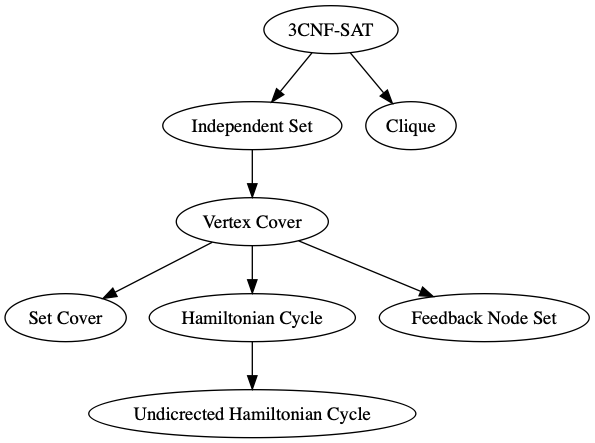
\includegraphics[scale=0.4]{../figures/reductions.png}
\caption{Name}
\end{figure}

\subsection*{DigitsInBase}
This entry of Archive of Formal Proofs shows the uniqueness of representation of natural numbers given an arbitrary base. In other words, it proves the well-definedness of the n-ary counting systems. Our implementation benefits from this repository in showing the correctness of the polynomial reduction from \XC\ to \Part.

\section{NP-Hardness and polynomial reductions}
\subsection{Decision problems}
We may encounter many real-life problems that require a decision process to find a solution. When shopping at a supermarket, for example, we always want to choose the shortest queue. Another example is board games like go and chess. These problems are formally defined as decision problems. \\\\
A decision problem is a yes-no question on an infinite set of fixed type of inputs. Generally, if we refer to a decision problem $A$, we are referring to the set of all inputs for which the answer to the yes-no question is yes. The handling of a decision problem usually involves two questions:
\begin{enumerate}
    \item Is there an algorithm, which computes the solution to this problem, terminating on all inputs?
    \item If the answer to the first question is yes, is this algorithm efficient?
\end{enumerate}
If the answer to the first question is yes for a problem, it is a decidable problem, otherwise it is non-decidable. We do not expect a yes or no answer for the second question, but would like to find the optimal complexity for the algorithm. If there is a non-deterministic algorithm that decides the solution to the problem in polynomial time, it is in the complexity class \NPH.
Thus, we would like to know if the deterministic algorithms to compute the \NPH\ problems have a polynomial complexity.

\subsection{Polynomial reductions}
Given two decision problems $A$ and $B$, 
a reduction is a function $f: A \rightarrow B$, 
which maps the inputs of the question of the first problem 
to that of the second problem. A reduction is polynomial 
if and only if the reduction function has a polynomial bound. 
For a polynomial reduction from $A$ to $B$, we writes $A \red B$. \\ \\
Let $M$ and $N$ denotes the domains of $A$ and $B$ respectively. 
A function $g: M \rightarrow N$ is a polynomial reduction 
if and only if the following conditions are fulfilled.
\begin{align}  
    &x \in A \iff g(x) \in B \\
    &\exists k\in \mathbb{N}. f \in \mathcal{O}(n^k)
\end{align}
For the convenience reason, we usually separate (2.1) into the soundness and completeness of the reduction.
\begin{align}
    soundness: \quad x \in A \Longrightarrow g(x) \in B \\
    completeness: \quad g(x) \in B \Longrightarrow x \in A
\end{align}

\subsection{NP-Hardness and \SAT}
To show a decision problem $B$ is \NPH, 
we have to find a \NPH\ problem and polynomial reduction 
s.t. $A \red B$. A first proven \NPH\ problem is \SAT, 
which was independently proven by Cook in 1971 and Levin in 1973. 
The \SAT\ problem is denoted by 
\problem{\SAT}{A propositional logical formula in 
conjunctive normal form. }{Is there a valid assignment for this formula?}
However, for formal verification, we still need a formal definition using mathematical terms. In the previous implementation of the project, the \SAT\ is defined by a list of clauses, with the clauses as the sets of variables.
\begin{align*}
    \text{TODO: Replace this with Isabelle output.}
\end{align*}
There have been many attempts to solve \SAT\ problem in a polynomial bound, as well as many approaches to solve \SAT\ problem efficiently in certain scenarios. Thus, \SAT\ is one of the most studies \NPH\ problems, from which there are also many \NPH\ problems reduced. Our first reduction also stems from \SAT, while all the other reductions are constructed upon novel introduced problems. More details on the reduction and implementation are given in Chapter 3 and Chapter 4. 
